\part{Medical Image Visualization}

Medical image visualization encompasses the entire process of displaying and presenting medical images and related information to facilitate diagnosis and clinical decision-making. It's a multidisciplinary field drawing on science and engineering, including computer sciences, medical physics, and perceptual psychology

Visualization should allow a physician to the interpret the images for accurate diagnosis

Contrast Resolution: This is the ability to detect very subtle changes in grayscale and distinguish them from image noise. It's primarily characterized by the signal-to-noise ratio (SNR) in an image

Quantum noise is common in X-ray or gamma ray images because relatively few quanta are used to limit patient radiation dose

Display should be calibrated.

The human eye perceives brightness differences non-linearly.

At low luminance, the eye is very sensitive → small changes in brightness are perceptually big.

At high luminance, the eye is less sensitive → bigger brightness jumps are needed to recognize a change in the luminance.

Luminance is measured with a photometer

The Barten model of human visual contrast sensitivity


\chapter{Perception}

\section{Perception of the luminance VS the luminance}
\begin{itemize}
\item The perception of the intensity is not linear.
\end{itemize}
\begin{center}
  
\includegraphics[width=0.9\textwidth]{linear2}\\
  (In each row and column, the gradient is linear.)
\end{center}

\section{Perception of the luminance VS the frequency}
\begin{itemize}
\item The perception of a change of the intensity varies with the spatial frequency.
\end{itemize}
\begin{center}
  
\includegraphics[width=0.65\textwidth]{CSF3}\\
  (\gls{CSF}.)
\end{center}

\section{Perception of the \popup{luma}{Luminance.} VS the neighborhood (1/2)}
\begin{itemize}
\item The perception of the intensity depends the neighbour pixels.
\end{itemize}
\begin{center}
  
\includegraphics[width=0.8\textwidth]{linear3}\\
  (In each block, all the pixels have the same intensity.)
\end{center}

\section{Perception of the \popup{luma}{Luminance.} VS the neighborhood (2/2)}
\begin{itemize}
\item The perception of the intensity depends the neighbour pixels.
\end{itemize}
\begin{center}
  
\includegraphics[width=1.0\textwidth]{contraste_simultaneo}\\
  (All the internal squares have the same intensity.)
\end{center}

\section{Perception of the luma VS the visualization time}
\begin{itemize}
\item The perception of the intensity depends the visualization time.
\end{itemize}
\begin{center}
  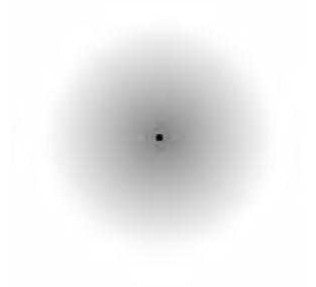
\includegraphics[width=0.4\textwidth]{punto_y_difuminado}\\
  (Look to the central point for a while.)
\end{center}

\section{Noise masking}
\begin{itemize}
\item The perception of the structures depends on the type and intensity of the noise.
\end{itemize}
\begin{center}
  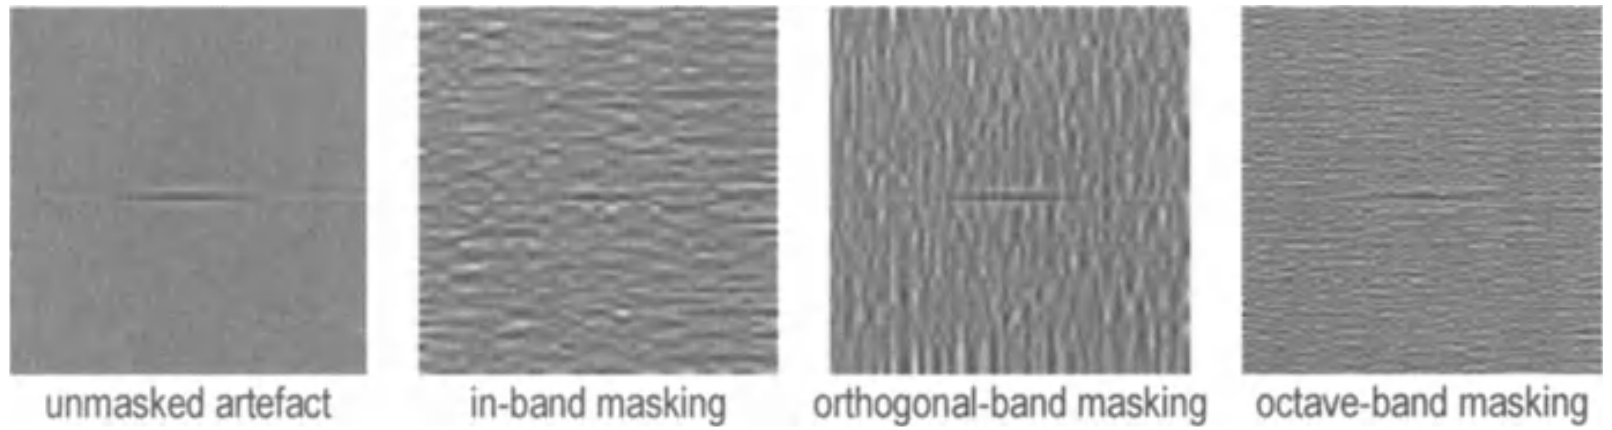
\includegraphics[width=1.0\textwidth]{noise_masking}\\
  (Different effects of Gaussian noise in the Wavelet domain.)
\end{center}
